% IEEE conference-format draft. Source of truth for the text: docs/PAPER_DRAFT.md.
% Build: tectonic docs/paper/main.tex   (or upload docs/paper/ + figures/ to Overleaf)
\documentclass[conference]{IEEEtran}
\usepackage{graphicx}
\usepackage{booktabs}
\usepackage{amsmath}
\usepackage{xcolor}
\usepackage{url}
\usepackage[hidelinks]{hyperref}
\graphicspath{{../../figures/}}
\newcommand{\team}[1]{{\color{red}\footnotesize[TEAM: #1]}}

\begin{document}

\title{Degradation-Aware Training, Not Frequency-Band Decomposition, Makes Brain Tumor Segmentation Robust to Simulated Low-Field MRI}

\author{\IEEEauthorblockN{Joshua Koshy, Muhammad Nazir Ahmed Mapkar, Mayank \team{full names, order, affiliations}}
\IEEEauthorblockA{ECTE408 \team{institution}}}

\maketitle

\begin{abstract}
Low-field MRI could widen access to brain imaging, but its scans are noisier and blurrier than the high-field
data segmentation networks are trained on. We tested whether splitting each image into low- and
high-spatial-frequency bands, processed in separate network streams, makes brain tumor segmentation more robust
to this degradation than conventional training on degraded data. On BraTS 2020 (258 training, 37 validation, 74
test patients) we simulated low-field acquisition in k-space: band-limited complex noise at SNR 8, 5 and 3,
halved in-plane resolution and 5~mm slices, giving 13 conditions including clean. Five capacity-matched 2D
U-Nets were each trained with three seeds: a clean-trained baseline (M0), a U-Net trained on degraded data (M1),
a dual-stream frequency-band network (M4), a low-band-only ablation (M5) and an early-fusion variant (M6). Three
hypotheses comparing M4 with M1 and M6 were pre-registered before training. Training on degraded data was the
decisive factor: at the worst condition the augmented models reached a mean 3D Dice of 0.763--0.769 against
0.549 for the baseline, and removed its spurious tumor on tumor-free slices (0.4 vs 19.8~cm$^3$), about a
quarter of which lay outside the brain. None of the pre-registered hypotheses was supported: the dual-stream
network did not beat the plain augmented U-Net or early fusion (differences $-0.004$, below twice the
seed-to-seed SD). Tumor volumes of the augmented models stayed as reliable at the worst condition as on clean
scans (median whole-tumor error about 7\%, ICC 0.93--0.94); the baseline's error rose to 26\% (ICC 0.74) while
its mean bias stayed near zero.
\end{abstract}

\begin{IEEEkeywords}
low-field MRI, brain tumor segmentation, robustness, data augmentation, frequency decomposition, U-Net, BraTS
\end{IEEEkeywords}

% ------------------------------------------------------------------------------------------------
\section{Introduction}

Magnetic resonance imaging is the reference modality for brain tumor diagnosis, treatment planning and
follow-up, but conventional 1.5--3~T scanners are expensive to buy, site and run, which concentrates them in
large hospitals in high-income settings~\cite{arnold2022lowfield,ogbole2018westafrica,anazodo2023camera}. In
West Africa, a survey found 84 MRI units for about 373 million people, most of Nigeria's being low-field
systems~\cite{ogbole2018westafrica}. Low-field systems (0.25--1~T~\cite{marques2019lowfield}; recent portable
scanners operate near 0.064~T~\cite{iglesias2023superres}) cost a fraction as much and can be brought to the
bedside~\cite{sheth2021portable}. The price is image quality: signal grows roughly with field strength, so a
low-field image has a lower signal-to-noise ratio (SNR), and scanners compensate with larger voxels, i.e.\ lower
resolution~\cite{marques2019lowfield}.

Tumor segmentation networks, typically U-Net variants~\cite{ronneberger2015unet}, are trained and benchmarked
almost entirely on high-field data such as BraTS~\cite{menze2015brats,bakas2017tcga}. Their accuracy must hold
up when SNR and resolution fall, and not only in overlap scores: tumor volumes derived from the segmentation
inform clinical decisions, so a model that keeps its Dice but mis-sizes tumors would still fail clinically.

Noise and resolution loss do not affect all spatial frequencies equally. Most image energy lies at low
frequencies (smooth contrast, overall tumor shape), while edges and fine detail sit at high frequencies, where
noise dominates first and resolution loss removes content outright. This motivates the hypothesis tested here:
separating each image into a low and a high band before the network, and processing them in separate streams,
might let the network rely on the robust low band when the high band becomes unreliable. The fair test of that
idea is not against a network trained on clean scans, which any degradation-trained model will beat, but
against the same training data fed to a conventional network.

Our contributions are: (i) a controlled comparison of five capacity-matched 2D U-Nets, three seeds each, under
13 simulated low-field conditions with noise restricted to the acquired k-space band; (ii) hypotheses, range
and protocol fixed in a dated decision log before training, with the comparison that isolates architecture
from training data as the primary test and a pre-specified training-noise rule; (iii) a clear negative result
for frequency-band decomposition; (iv) morphometric validation of tumor volume and shape with agreement
analysis validated on synthetically damaged masks; and (v) an independent MATLAB re-implementation of the
physics, numerically matched to the Python code.

% ------------------------------------------------------------------------------------------------
\section{Related Work}

\textit{Low-field MRI.} Most computational work on low-field images repairs the image before analysis; Iglesias
et al.\ synthesised 1~mm images from 0.064~T scans with a super-resolution network so standard morphometry tools
could be applied~\cite{iglesias2023superres}. That work concerns brain anatomy, not tumors; we found no
glioma-segmentation evaluation on low-field scans.

\textit{Tumor segmentation.} BraTS~\cite{menze2015brats,bakas2017tcga,bakas2018brats} underpins glioma
segmentation; inter-rater Dice for tumor sub-regions lies between 74\% and 85\%~\cite{menze2015brats}. The
self-configuring nnU-Net~\cite{isensee2021nnunet} won BraTS 2020 with region-based training and heavier
augmentation~\cite{isensee2020bratsnnunet}.

\textit{Robustness.} Performance loss under acquisition shift is well documented~\cite{karani2021testtime}.
Remedies include simulating the expected shift by augmentation~\cite{zhang2020bigaug}, test-time
adaptation~\cite{karani2021testtime} and image restoration~\cite{iglesias2023superres}. In natural images,
Gaussian-noise augmentation improves robustness to high-frequency corruptions but can reduce it for
low-frequency ones~\cite{yin2019fourier}; our degradation is mostly of the first kind.

\textit{Frequency-aware networks.} CNN generalisation has been linked to high-frequency image
content~\cite{wang2020highfreq}, frequency-domain inputs can improve classification~\cite{xu2020frequency}, and
medical segmentation networks add spatial-frequency attention~\cite{zhou2024sfunet} or, closest to our design,
split brain MRI into low- and high-frequency components processed separately~\cite{shao2025hffnet}. These are
evaluated on standard-quality data; none tests whether the decomposition helps under controlled degradation.

\textit{Volumetric agreement.} Response assessment relies largely on 2D measurements~\cite{wen2010rano}, which
motivates automated volumetry~\cite{kickingereder2019automated,chang2019autorano}. Agreement should be judged
with limits of agreement~\cite{bland1986agreement} and an ICC form matched to the design~\cite{shrout1979icc},
not correlation alone.

% ------------------------------------------------------------------------------------------------
\section{Methods}

\subsection{Data}
We used the BraTS 2020 training set~\cite{menze2015brats,bakas2017tcga,bakas2018brats}: 369 pre-operative glioma
patients (293 HGG, 76 LGG), four co-registered skull-stripped sequences (T1, T1ce, T2, FLAIR) at 1~mm isotropic
on a $240\times240\times155$ grid, with labels for necrotic core, edema and enhancing tumor, evaluated as whole
tumor (WT), tumor core (TC) and enhancing tumor (ET). Patients were split once, stratified by grade, into
training (258), validation (37) and test (74; 59 HGG, 15 LGG). All development used validation patients; the
test set was evaluated once, after all models were trained. Slices were cropped to $192\times192$; no test
patient has tumor outside the crop, and the label maps written by the evaluation pipeline match the raw
segmentations voxel for voxel.

\subsection{Simulated Low-Field Degradation}
Degradation is applied to raw intensities of each sequence in three steps. \emph{Slice thickness:} a $t$~mm slice
is the mean of $t$ consecutive 1~mm slices (centred, edges replicated), kept on the 1~mm grid. \emph{In-plane
resolution:} each slice is Fourier transformed and only the central fraction $r$ of k-space along each axis is
kept (pseudo-k-space truncation of the magnitude image). \emph{Thermal noise inside the acquired band:} complex
Gaussian noise $n$ is restricted to the same k-space mask $M_r$ and rescaled by $1/\sqrt{f}$ ($f$ the kept
fraction) so its per-pixel SD stays $\sigma$; the degraded image is
\begin{equation}
x_{\mathrm{deg}} = \left|\,\mathcal{F}^{-1}(M_r\cdot\mathcal{F}x) + \sigma\, n_{\mathrm{band}}\right|,
\qquad \sigma = \mu_{\mathrm{brain}}/\mathrm{SNR},
\end{equation}
which gives Rician tissue and Rayleigh background statistics~\cite{gudbjartsson1995rician}; $\mu_{\mathrm{brain}}$
is the mean clean brain intensity of that patient and sequence, and SNR is a linear ratio. The 13 conditions are
SNR $\in\{8,5,3\}\times r\in\{1.0,0.5\}\times t\in\{1,5\}$~mm plus clean; the worst is SNR~3, $r$~0.5, 5~mm. The
range was fixed in a validation pilot before training: every noisy condition cost a separately trained clean
baseline at least 0.17 Dice, so a robustness gain would be detectable. For validation and test, noise is seeded
per (patient, condition) by SHA-256 hashing, so every model sees identical degraded volumes. Fig.~\ref{fig:diag}
shows a clean and a worst-condition slice.

\subsection{Frequency-Band Decomposition}
Each degraded, brain-z-scored slice is split with complementary Gaussian filters in the centred Fourier domain,
$H_{\mathrm{lp}} = \exp(-D^2/2D_0^2)$ and $H_{\mathrm{hp}} = 1 - H_{\mathrm{lp}}$, with $D$ the radius normalised
to Nyquist and $D_0 = 0.20$. The bands sum exactly to the input (reconstruction error $5\times10^{-7}$), so the
split discards no information. $D_0$ was fixed as a design choice motivated by the spectral analysis
(Section~\ref{sec:spectral}), where 92--97\% of clean-image power lies below it; an early search over
$D_0 \in \{0.10, 0.15, 0.20, 0.30\}$ on three validation patients was too weak to select it empirically, and
other cutoffs were not tested.

\subsection{Models and Training}
All models are 2D U-Nets with five levels, instance normalisation and LeakyReLU, outputting sigmoid WT, TC and
ET channels, with parameter counts matched within 4.5\% (Table~\ref{tab:models}). The decomposition is part of
the model for M4--M6. M1 vs M0 isolates training data; M4 vs M1 the band-split architecture with data held fixed;
M4 vs M6 two streams vs one given the same bands; M5 vs M4 the contribution of the high band. Three further
planned configurations reduced to duplicates of M1, M5 and M4 as implemented and were dropped.

Every model was trained for 20 epochs on all brain slices of the training patients (12{,}000 random slices per
epoch, batch 32, AdamW $3\times10^{-4}$ with warm-up and cosine decay, BCE plus batch soft Dice, flips, mixed
precision), with seeds 0, 1 and 2. M1, M4, M5 and M6 draw one of the 13 conditions uniformly per training slice;
M0 sees clean slices. The checkpoint with the highest mean full-volume validation Dice over three conditions
(clean; SNR~5; worst) was kept, the same rule for every model. Inference thresholds sigmoid outputs at 0.5 on
full volumes. An earlier protocol that trained on tumor-bearing slices only failed on full volumes and is not
used.

\begin{table}[t]
\caption{Models (parameter counts matched within 4.5\%)}
\label{tab:models}
\centering\footnotesize
\resizebox{\columnwidth}{!}{\begin{tabular}{@{}llll@{}}
\toprule
Model & Design & Training data & Params \\
\midrule
M0 & U-Net & clean & 4.37\,M \\
M1 & U-Net & degraded & 4.37\,M \\
M4 & dual-stream U-Net (low/high encoders) & degraded & 4.17\,M \\
M5 & U-Net on low band only & degraded & 4.37\,M \\
M6 & U-Net, low + high as 8 channels & degraded & 4.37\,M \\
\bottomrule
\end{tabular}}
\end{table}

\subsection{Hypotheses and Statistics (Pre-registered)}
Tests use full-volume 3D Dice averaged over WT, TC and ET, seed-averaged per patient, on the 74 test patients.
\textbf{H1} (primary): at the worst condition, M4 $>$ M1. \textbf{H2}: M4's clean-to-worst drop is smaller than
M1's. \textbf{H3}: at the worst condition, M4 $>$ M6. Each is a two-sided paired Wilcoxon signed-rank
test~\cite{wilcoxon1945ranking} with Holm correction~\cite{holm1979sequential}, $\alpha = 0.05$. A hypothesis is
supported only if the difference is significant, in the predicted direction and at least twice the seed-to-seed
SD (SD across seeds of a model's patient-averaged Dice, larger of the two models). Secondary comparisons (M4 vs
M0, M5 vs M4) are reported outside the verdict. Effect sizes use 95\% percentile bootstrap intervals over
patients (10{,}000 resamples). We also report HD95 with the BraTS empty-mask convention and false-tumor volume
(predicted WT on slices without tumor).

\subsection{Morphometrics and Agreement}
For seed-0 predictions at clean, SNR~5 and worst, and for the ground truth, identical MATLAB code computes per
region the volume, surface area (per connected component, cross-checked with a smoothed marching-cubes
mesh~\cite{lorensen1987marching}), sphericity~\cite{wadell1935volume}, elongation and connected-component count.
Agreement is reported as volume error, Bland-Altman bias and 95\% limits~\cite{bland1986agreement}, and
ICC(A,1)~\cite{mcgraw1996icc,shrout1979icc} with bootstrap intervals. The pipeline was validated on the test
ground truths with known synthetic damage (dilation, erosion, shift, deleted and spurious blobs) before use.

\subsection{Implementation Verification and Spectral Analysis}
\label{sec:spectral}
The degradation was re-implemented independently in MATLAB and compared with the Python function used for
training and evaluation on identical inputs and noise for all 13 conditions; the largest difference was
$1.1\times10^{-6}$ of the mean brain intensity (float32 rounding). The MATLAB decomposition matched the PyTorch
code on five random slices for all four cutoffs with a maximum absolute difference of $4.8\times10^{-7}$
(intensities in $[0.1, 1]$). Two independent 3D renderers
(MATLAB and Python) agree on the surface-error measure within 0.5~mm on the cases of Fig.~\ref{fig:viz3dA}.

On the largest-tumor slice of 12 test patients, 95.1\% (FLAIR) and 91.9\% (T1ce) of clean spectral power lies
below $D_0 = 0.20$ (excluding DC). Under degradation (Fig.~\ref{fig:spectral}) the low band keeps more anatomy
than error at every condition (6--16~dB), while the high band falls below 0~dB from SNR~5 on, reaching about
$-5$ to $-6$~dB at SNR~3. Noise sets the band SNR almost entirely; resolution loss costs the high band at most
about 2~dB. The premise of band separation therefore holds: where the clean-trained model fails, most of the
high band is degradation.

\begin{figure}[t]
\centering
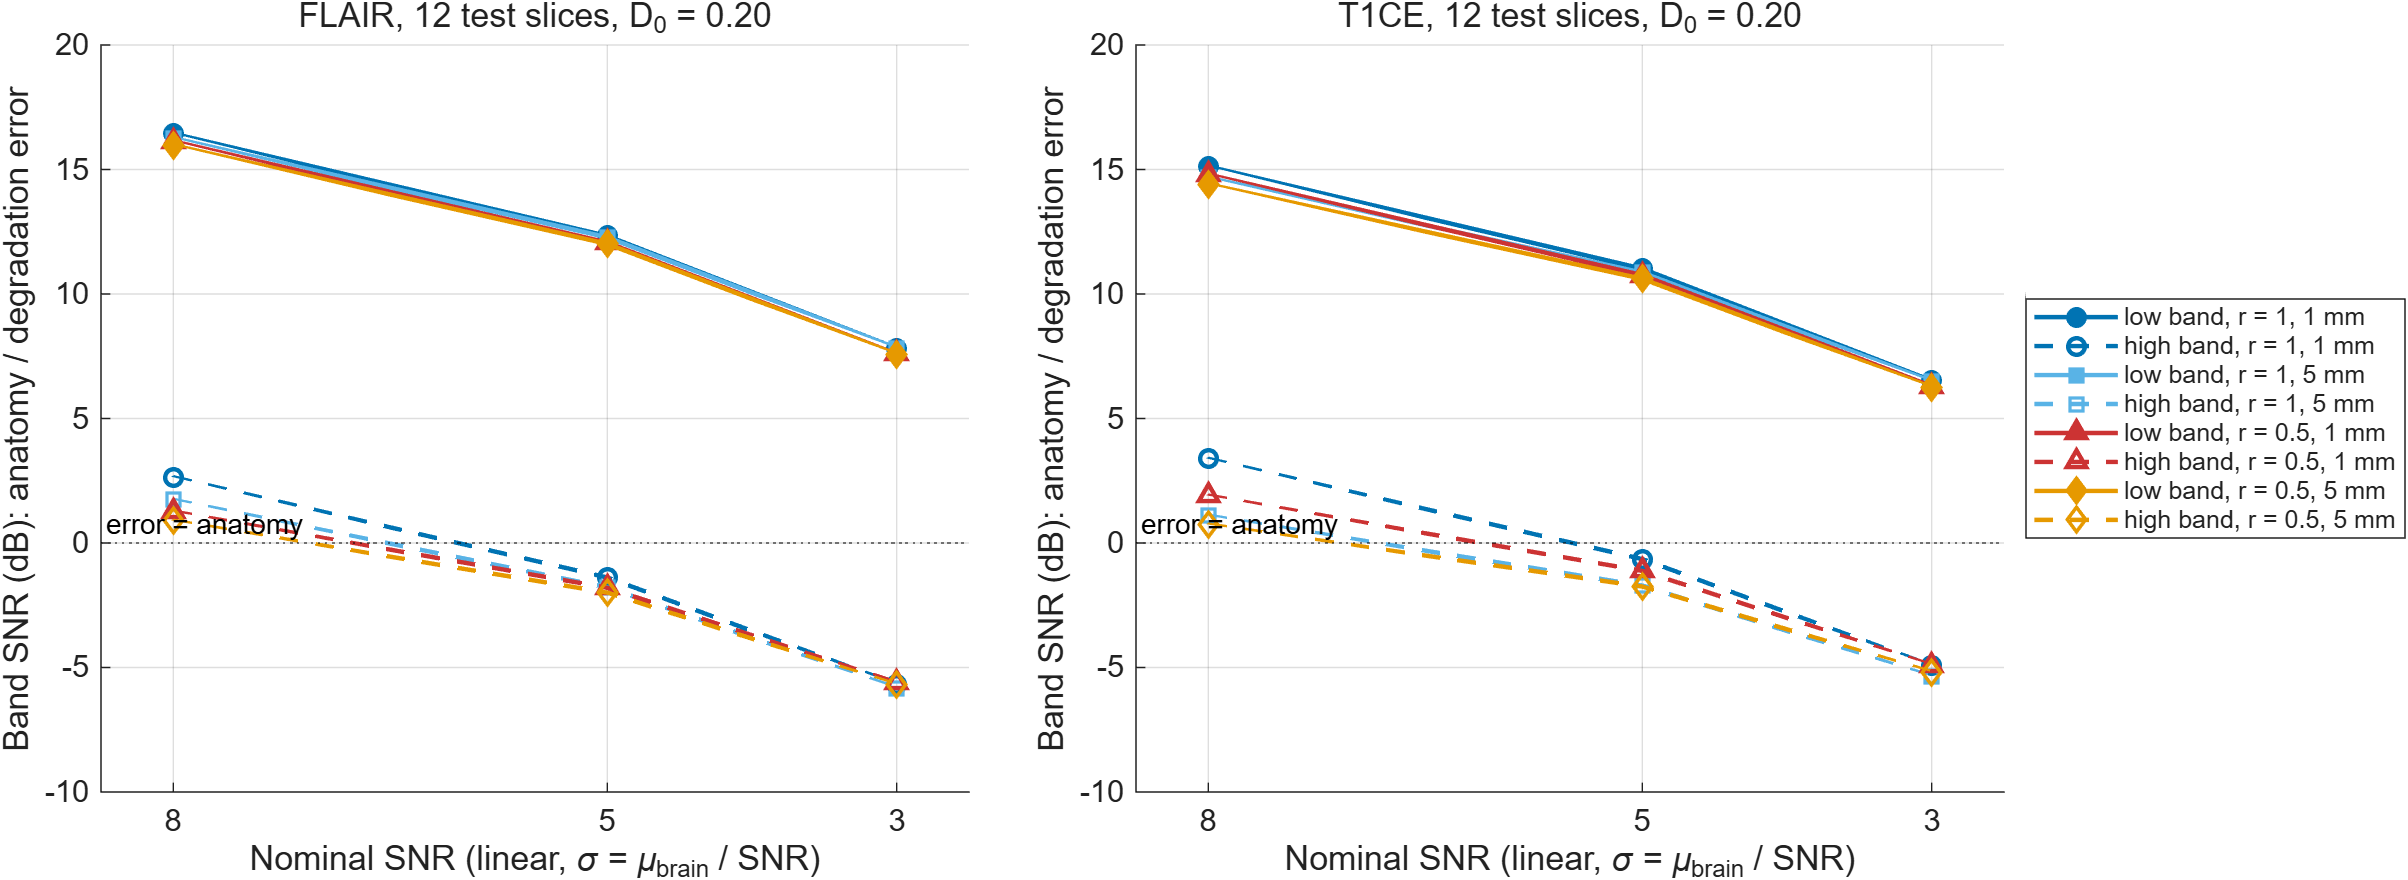
\includegraphics[width=\columnwidth]{spectral_band_snr.png}
\caption{Band SNR (clean anatomy power over degradation-error power, dB) in the low ($D<0.20$, solid) and high
(dashed) band for the 12 DEC-005 noisy conditions, FLAIR and T1ce, 12 test slices.}
\label{fig:spectral}
\end{figure}

% ------------------------------------------------------------------------------------------------
\section{Results}

\subsection{Accuracy Across Conditions}
Fig.~\ref{fig:dice} and Table~\ref{tab:dice} show mean 3D Dice per condition. The clean-trained M0 lost accuracy
under every degradation, and noise dominated: SNR~8 alone cost 0.099 Dice, SNR~3 a further 0.052, and halved
resolution with 5~mm slices another 0.086 (clean to worst: 0.237). The augmented models were almost insensitive
to noise (M1: 0.005 at SNR~8, 0.011 more at SNR~3); most of their remaining loss came from resolution at the
highest noise (clean to worst: 0.055--0.061). The four augmented models were within 0.012 of each other at every
condition and within 0.006 at the worst; M1 was best or tied everywhere. Per region at the worst condition, WT
was most robust (M1 0.863, M4 0.863, M0 0.702) and ET least (0.658, 0.653, 0.437).

\begin{figure}[t]
\centering
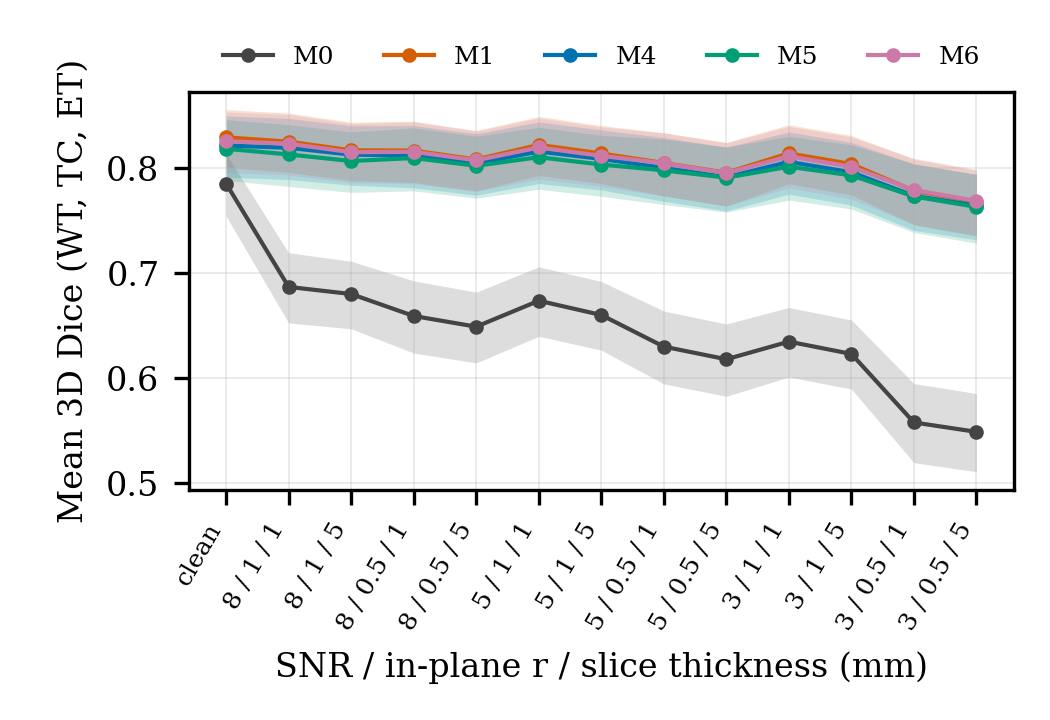
\includegraphics[width=\columnwidth]{dice_curves.png}
\caption{Mean 3D Dice (WT, TC, ET) per model across the 13 conditions, 74 test patients, seed-averaged; bands
are 95\% bootstrap CIs over patients.}
\label{fig:dice}
\end{figure}

\begin{table}[t]
\caption{Mean 3D Dice at selected conditions (all 13 in Fig.~\ref{fig:dice})}
\label{tab:dice}
\centering\footnotesize
\begin{tabular}{@{}lccccc@{}}
\toprule
SNR / $r$ / mm & M0 & M1 & M4 & M5 & M6 \\
\midrule
clean & 0.786 & 0.830 & 0.822 & 0.819 & 0.826 \\
8 / 1.0 / 1 & 0.687 & 0.825 & 0.820 & 0.813 & 0.823 \\
5 / 1.0 / 1 & 0.674 & 0.822 & 0.816 & 0.811 & 0.820 \\
3 / 1.0 / 1 & 0.635 & 0.814 & 0.806 & 0.802 & 0.812 \\
3 / 0.5 / 1 & 0.558 & 0.779 & 0.774 & 0.773 & 0.779 \\
3 / 0.5 / 5 (worst) & \textbf{0.549} & \textbf{0.768} & \textbf{0.765} & \textbf{0.763} & \textbf{0.769} \\
\bottomrule
\end{tabular}
\end{table}

\subsection{Pre-registered Hypotheses}
None of the hypotheses was supported (Table~\ref{tab:hyp}). For H1 and H3 the test was significant after
correction but in the opposite direction (M1 and M6 slightly better than M4), and the differences of about
0.004 are below a third of the training-noise threshold; we read them as no detectable difference. For H2 the
mean favours M4 and the median M1, and neither is significant.

\begin{table}[t]
\caption{Pre-registered tests at the worst condition (positive = M4 better)}
\label{tab:hyp}
\centering\footnotesize
\setlength{\tabcolsep}{3pt}
\resizebox{\columnwidth}{!}{\begin{tabular}{@{}llcccc@{}}
\toprule
& Test & Mean diff (95\% CI) & Holm $p$ & 2$\times$seed SD & Verdict \\
\midrule
H1 & M4 $>$ M1 & $-0.0037$ ($-0.0086$, $0.0004$) & 0.043 & 0.014 & not supp. \\
H2 & drop M4 $<$ M1 & $+0.0041$ ($-0.0008$, $0.0096$) & 0.70 & 0.005 & not supp. \\
H3 & M4 $>$ M6 & $-0.0044$ ($-0.0098$, $0.0001$) & 0.0017 & 0.014 & not supp. \\
\bottomrule
\end{tabular}}
\end{table}

\subsection{Secondary Comparisons, False Tumor and Stability}
At the worst condition M4 exceeded M0 by $+0.216$ Dice (95\% CI 0.195--0.237, Holm $p = 3\times10^{-13}$),
nine times the training-noise threshold; on clean scans $+0.036$, within training noise (M0's clean seed SD is
0.048). M5 matched M4 at both conditions ($-0.001$ and $-0.003$): discarding the high band cost nothing
measurable. Under noise M0 predicted 13--20~cm$^3$ of tumor on tumor-free slices, against 0.3--0.5~cm$^3$ for
every augmented model, and its median WT HD95 rose from 5.7 to about 100~mm while the augmented models stayed
below 5~mm. M0 was also the least reproducible model across seeds.

\textit{Where M0's false tumor lies.} The 3D renderings (Figs.~\ref{fig:viz3dA}--\ref{fig:viz3dB}) show much of
it outside the brain. On seed-0 predictions, 24\% of M0's predicted WT volume at the worst condition (23~cm$^3$
per patient) lay outside the brain mask, against under 1\% for the augmented models. No post-processing was
pre-specified; as a sensitivity analysis, masking predictions to the brain raises M0's seed-0 WT Dice from 0.78
to 0.88 at SNR~5 and from 0.65 to 0.76 at the worst condition, leaving the augmented models clearly better at the
worst condition (WT Dice $+0.10$, half the volume error). \team{masked M4 vs M0 test on all seeds: running, fill
in} The pre-registered comparisons are unaffected.

\subsection{Morphometric Agreement}
For the augmented models, tumor volume stayed about as reliable at the worst condition as on clean scans
(Table~\ref{tab:agree}, Fig.~\ref{fig:agree}): median absolute volume error 7.0--7.8\% for WT, 12.7--14.5\% for
TC and 17.1--18.5\% for ET, with limits of agreement widening by a few cm$^3$ and a slight WT underestimate
(bias $-4$ to $-6$~cm$^3$). M0's WT error rose from 5.8\% to 25.8\% and its ICC fell to 0.74, yet its mean bias
was $-0.2$~cm$^3$: spurious tumor and missed tumor cancel on average while per-patient errors reach about
$\pm73$~cm$^3$. A bias-only summary would have called M0 the most accurate model. Every model predicted ET in all
five test patients without ET.

\begin{table}[t]
\caption{WT volume agreement, seed 0, clean / worst condition}
\label{tab:agree}
\centering\footnotesize
\setlength{\tabcolsep}{3pt}
\resizebox{\columnwidth}{!}{\begin{tabular}{@{}lccc@{}}
\toprule
Model & Median abs.\ error (\%) & Bias (95\% LoA), worst, cm$^3$ & ICC(A,1) \\
\midrule
M0 & 5.8 / 25.8 & $-0.2$ ($-74$, $+73$) & 0.957 / 0.737 \\
M1 & 6.5 / 7.1 & $-5.8$ ($-42$, $+30$) & 0.956 / 0.938 \\
M4 & 6.8 / 7.0 & $-4.8$ ($-40$, $+31$) & 0.948 / 0.942 \\
M5 & 6.3 / 7.8 & $-5.3$ ($-45$, $+34$) & 0.947 / 0.928 \\
M6 & 6.8 / 7.2 & $-5.1$ ($-41$, $+31$) & 0.956 / 0.940 \\
\bottomrule
\end{tabular}}
\end{table}

\begin{figure*}[t]
\centering
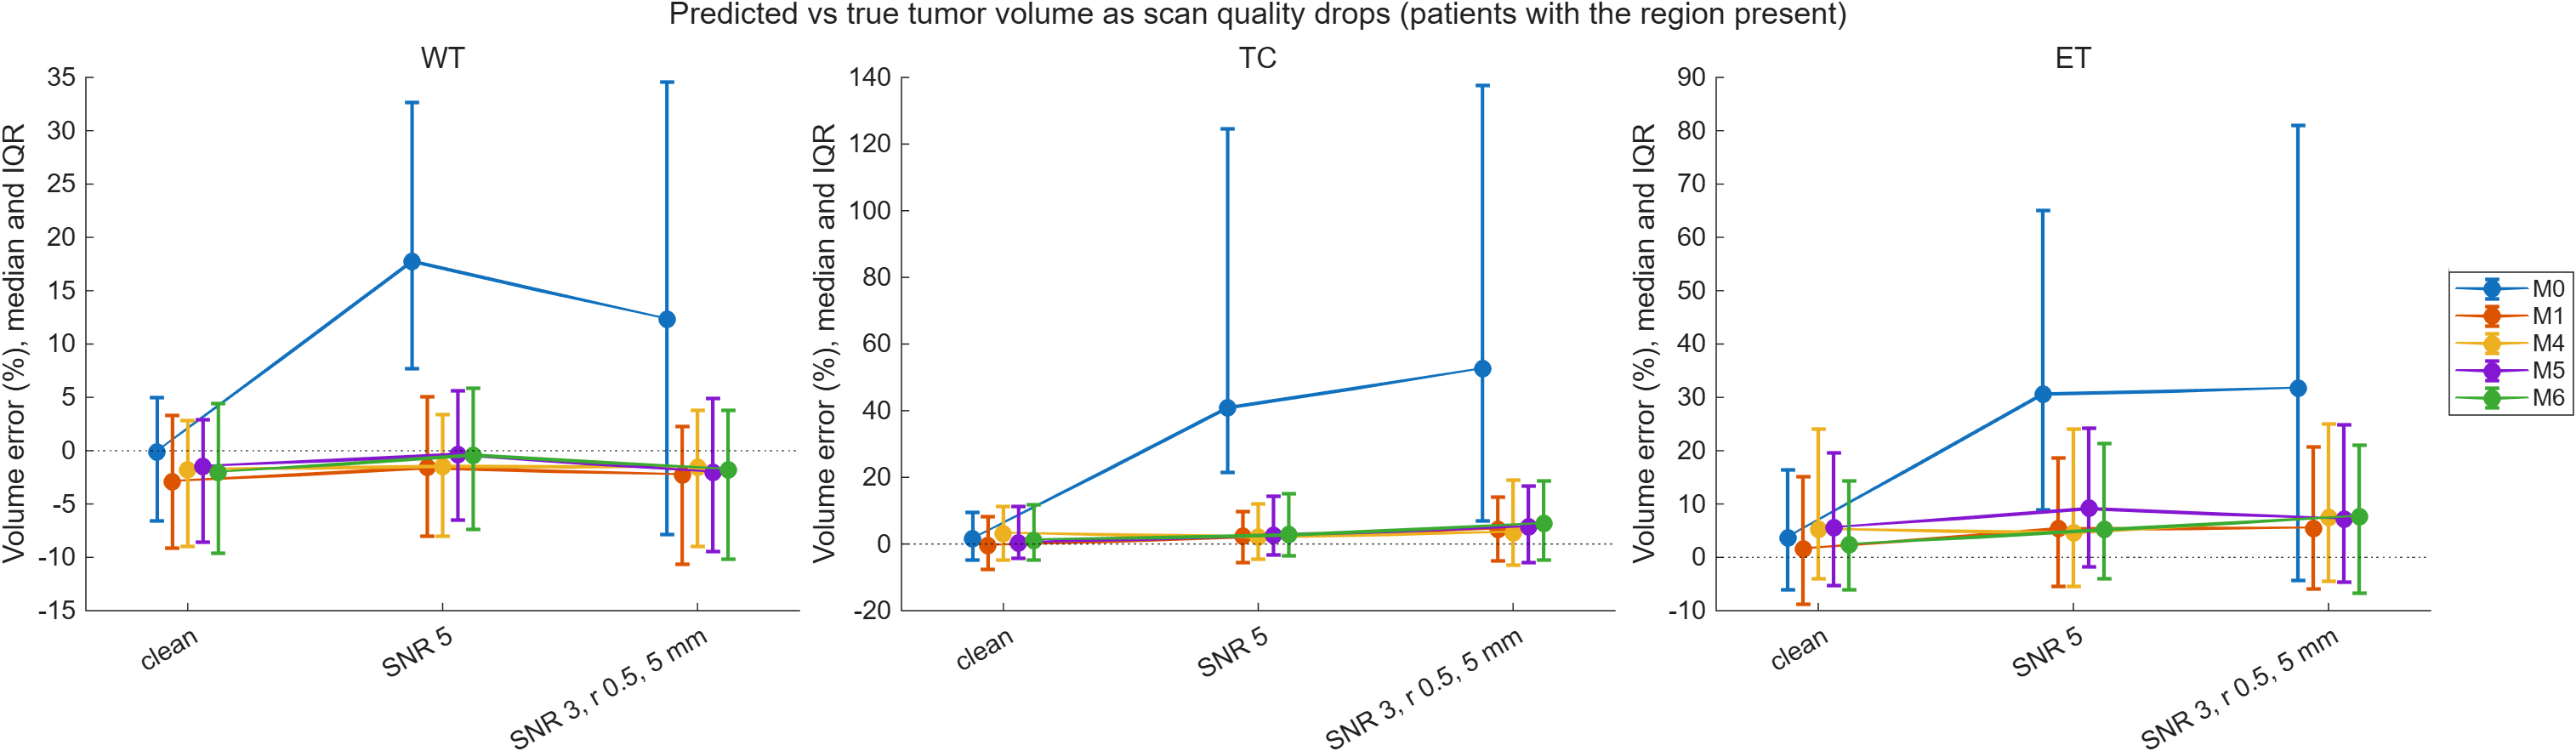
\includegraphics[width=0.49\textwidth]{agreement_stage3_volume_error.png}\hfill
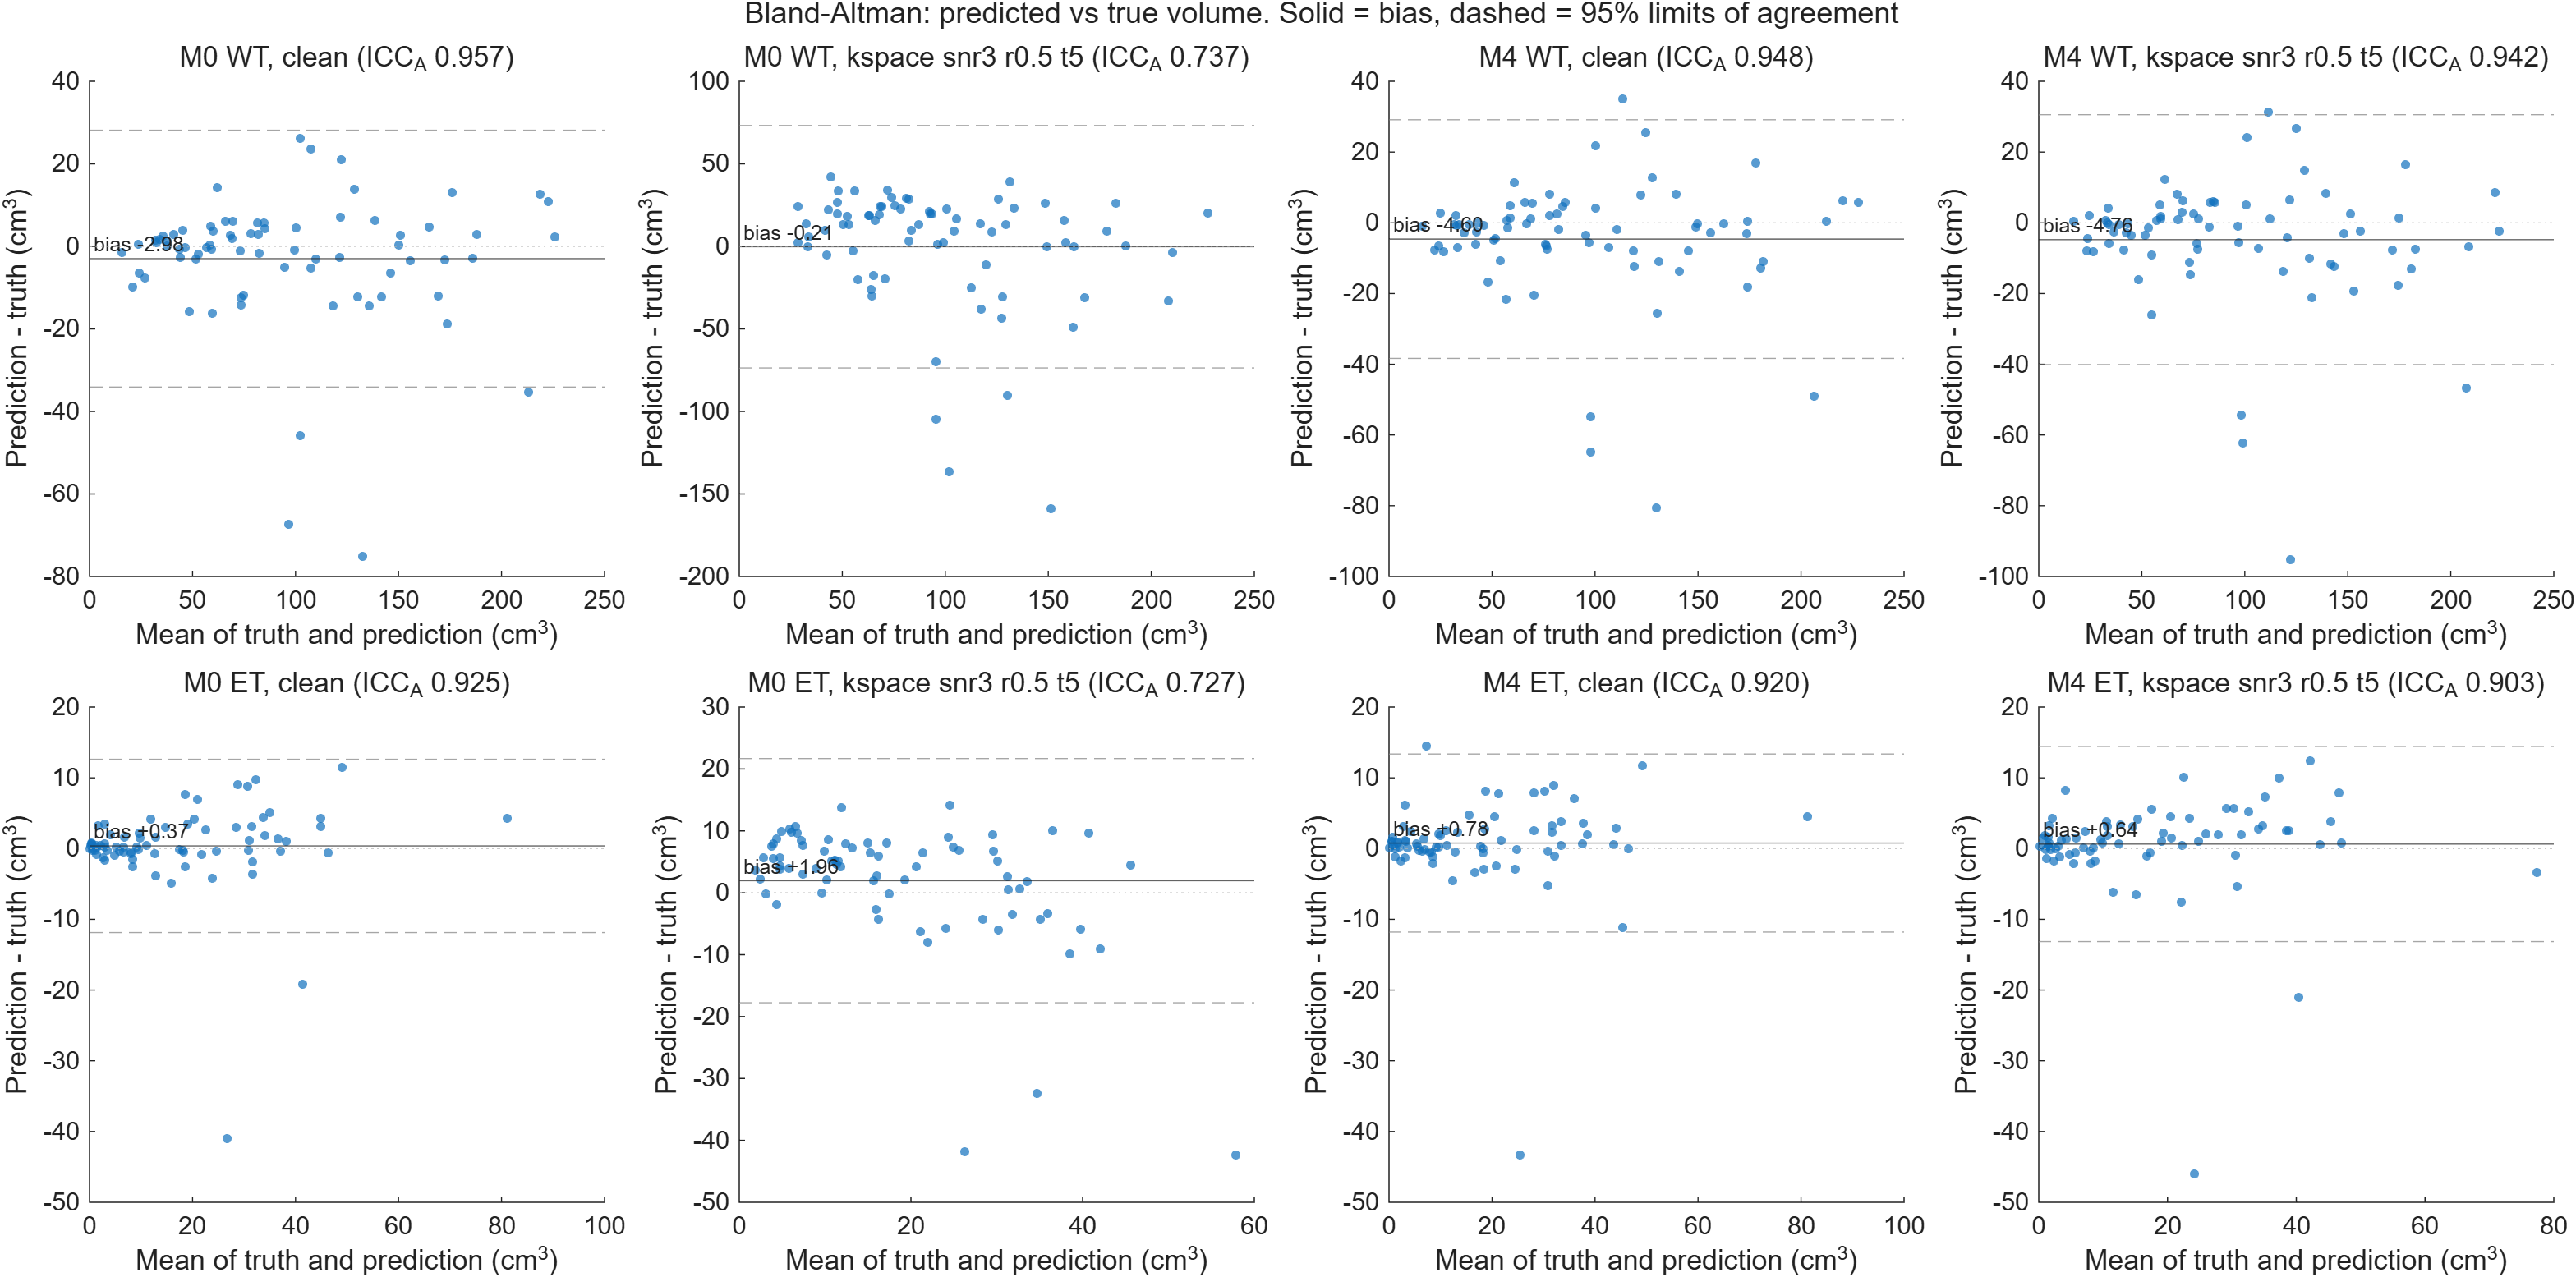
\includegraphics[width=0.49\textwidth]{agreement_stage3_bland_altman.png}
\caption{Left: median and IQR of predicted vs true volume error per region, model and condition (seed 0).
Right: Bland-Altman plots for M0 and M4, clean and worst condition, WT (top) and ET (bottom).}
\label{fig:agree}
\end{figure*}

\subsection{Qualitative Cases}
Five test patients were selected before any prediction was inspected, from ground truth only (HGG at the 10th,
50th and 90th volume percentile, LGG with and without ET). Fig.~\ref{fig:diag} shows the second; the 3D
comparisons of all five are in Figs.~\ref{fig:viz3dA}--\ref{fig:viz3dB}. In every case M0's predicted surface
is dominated by scattered islands, many outside the brain (mean surface distance 35--78~mm), while M4's follows
the true boundary (4--8~mm) apart from a few small specks. Two cases are hard for every model: the largest tumor,
whose core is under-segmented even on clean scans, and the LGG without ET, where predicted ET pulls the mean Dice
down although WT Dice is 0.84.

\begin{figure*}[t]
\centering
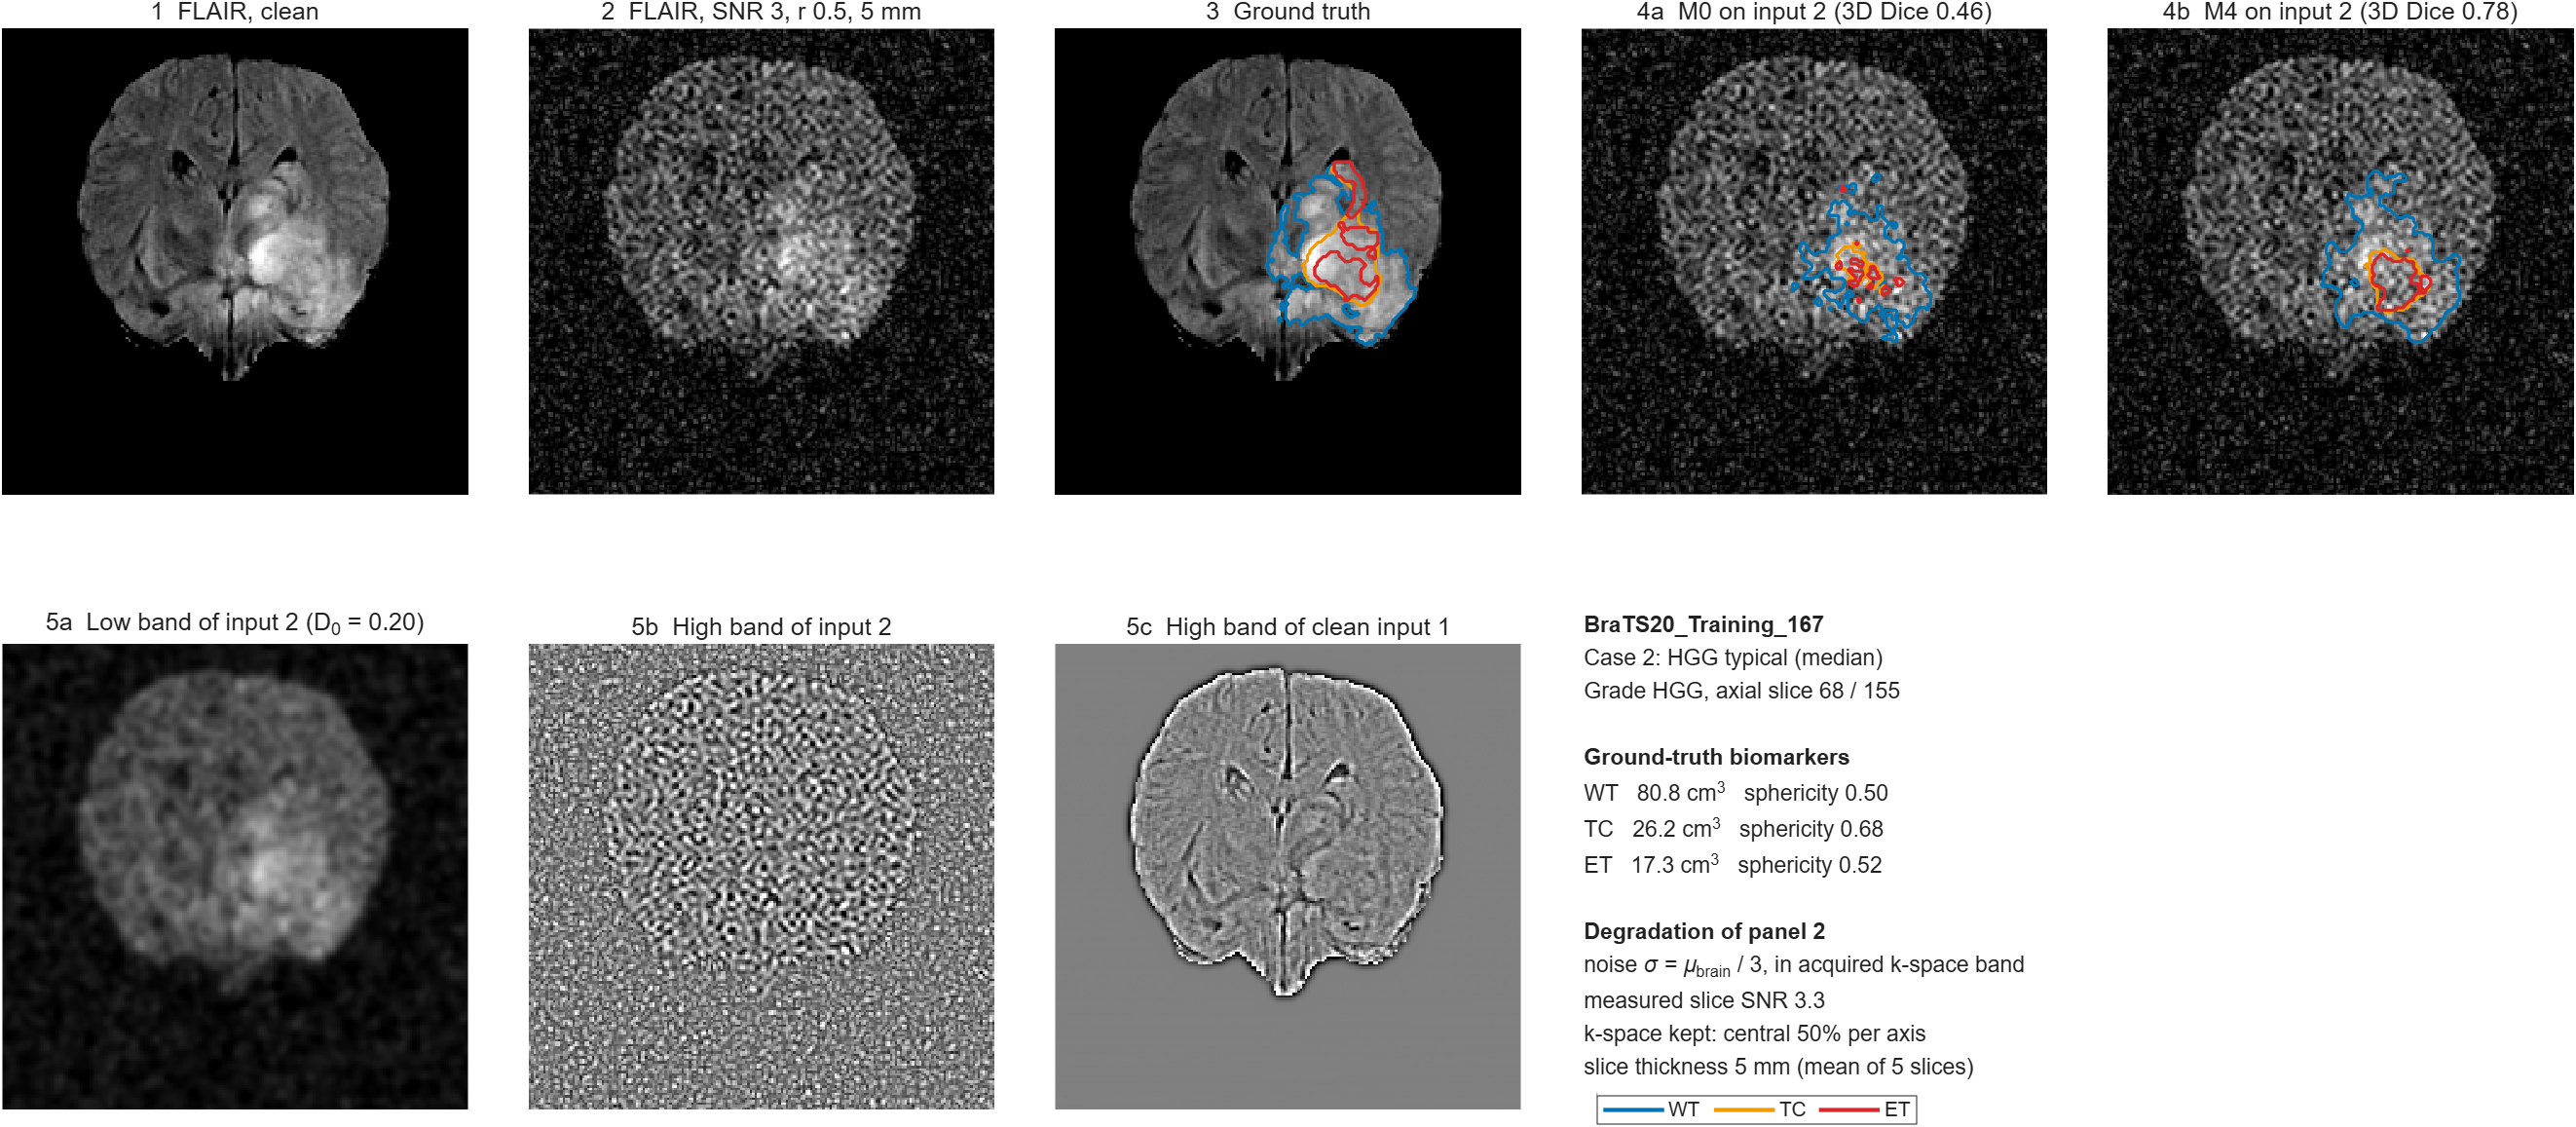
\includegraphics[width=\textwidth]{diagnostic_2_BraTS20_Training_167.png}
\caption{Case 2 (typical HGG). (1) clean FLAIR; (2) worst condition (SNR 3, $r$ 0.5, 5~mm); (3) ground truth;
(4a,b) M0 and M4 predictions on input 2 (WT blue, TC orange, ET red); (5a--c) low and high band of input 2 and
high band of the clean input.}
\label{fig:diag}
\end{figure*}

\begin{figure*}[t]
\centering
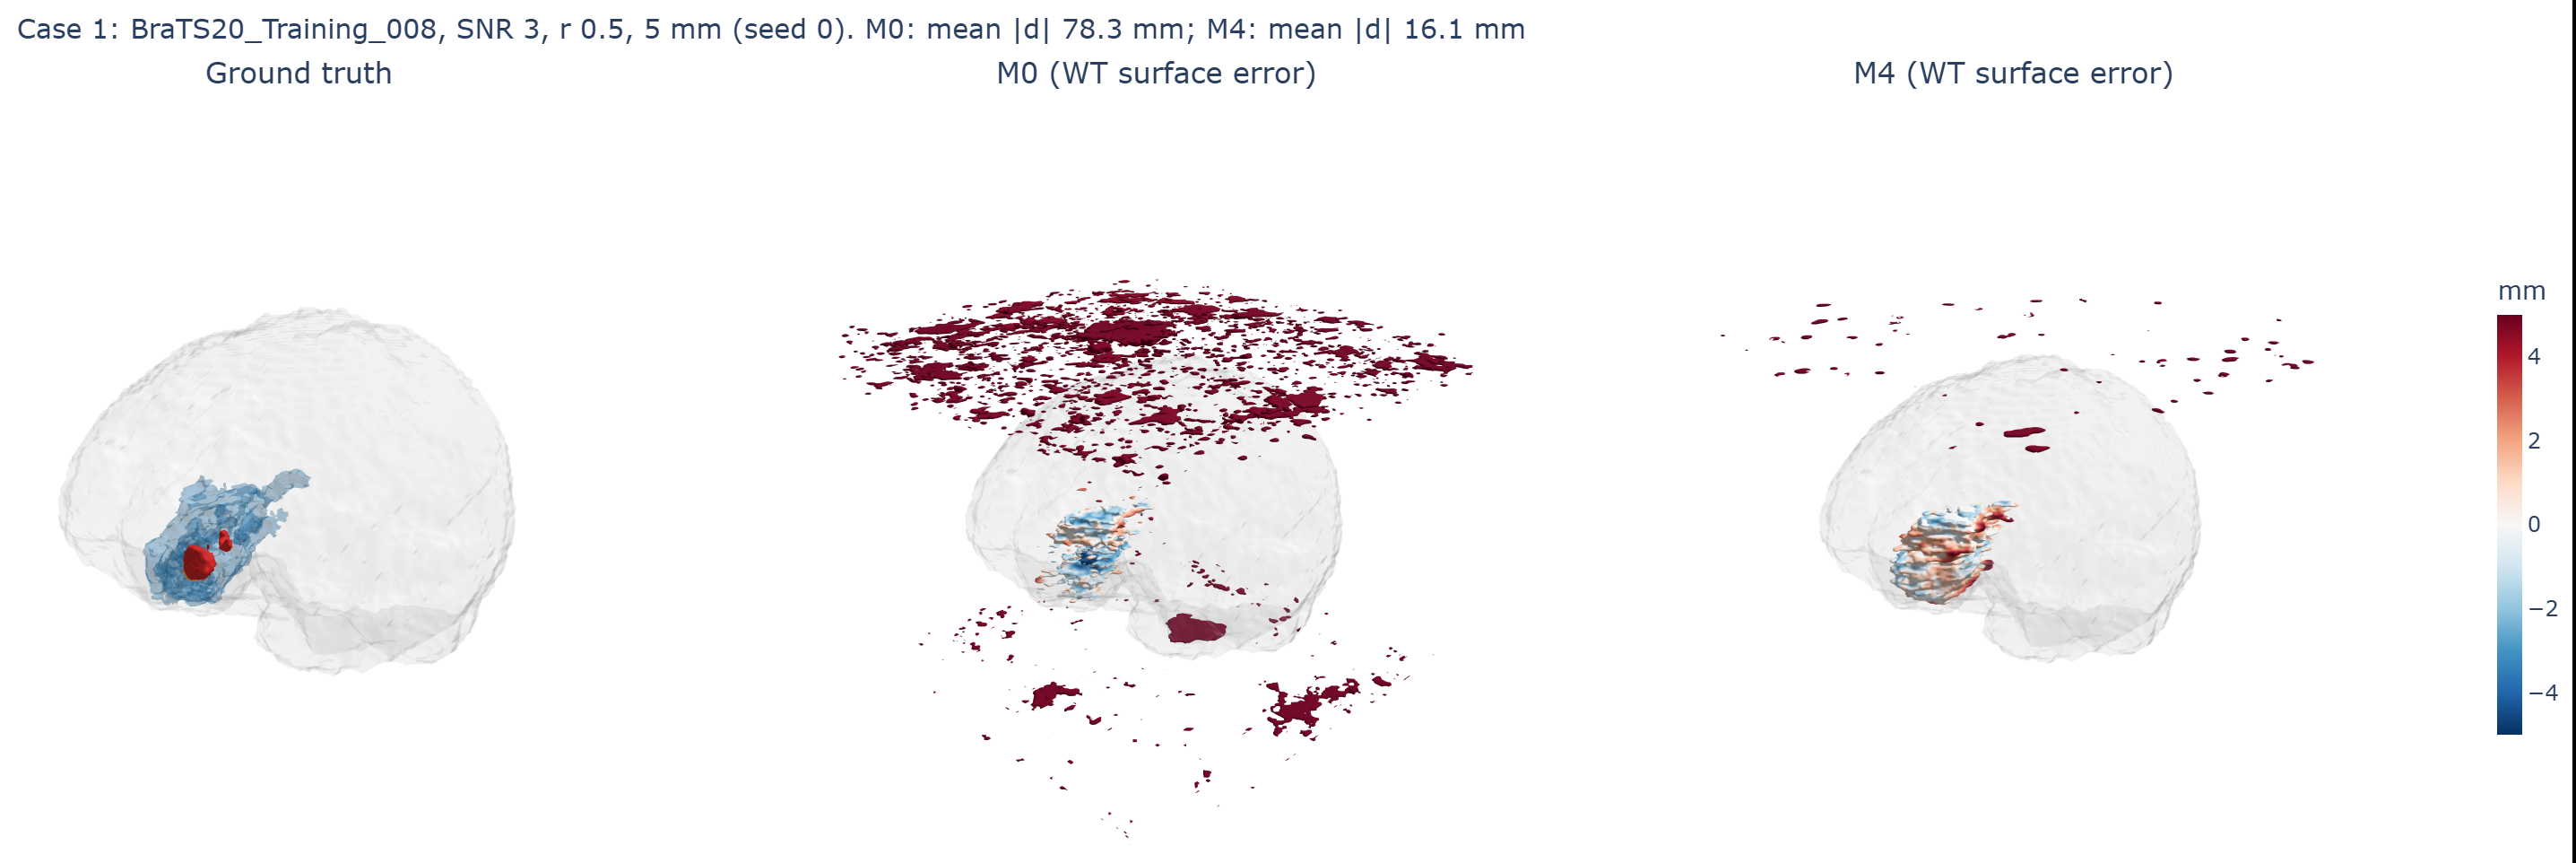
\includegraphics[width=\textwidth]{viz3d_case1_BraTS20_Training_008.png}\\[2pt]
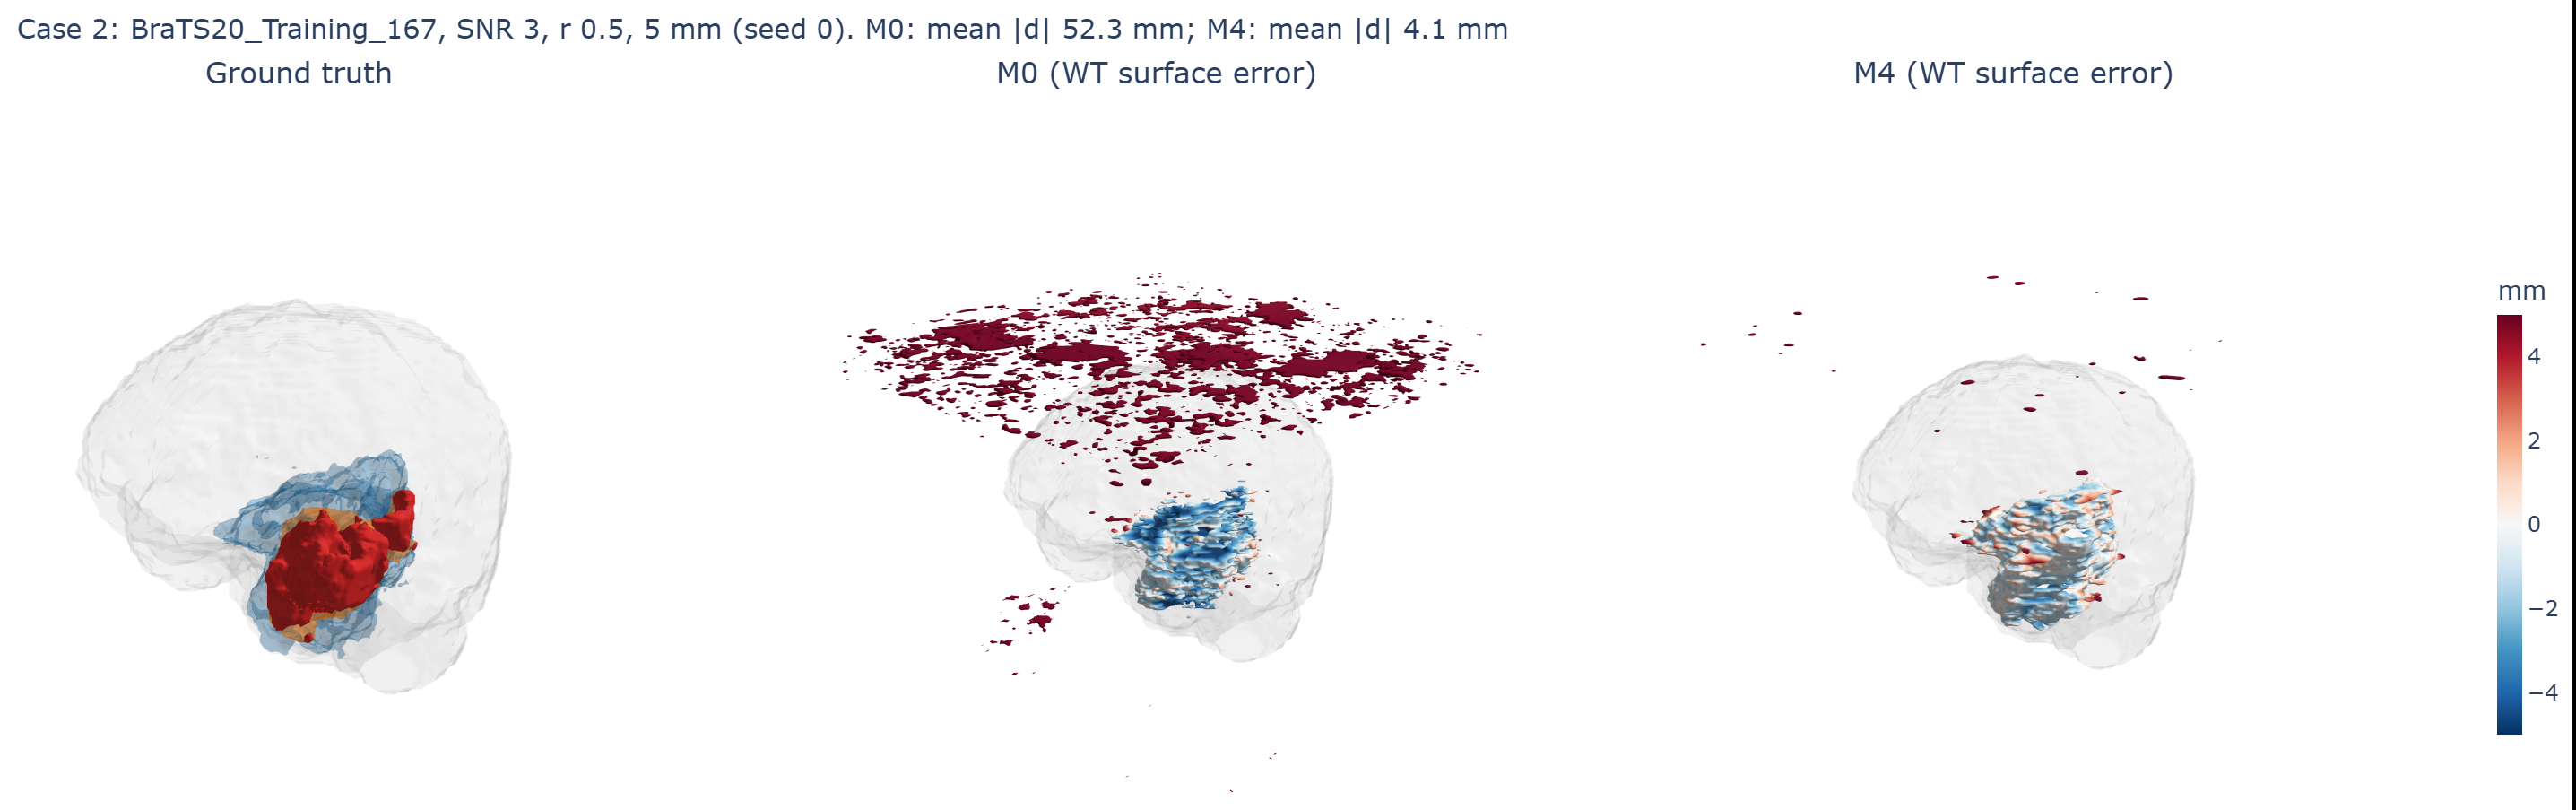
\includegraphics[width=\textwidth]{viz3d_case2_BraTS20_Training_167.png}\\[2pt]
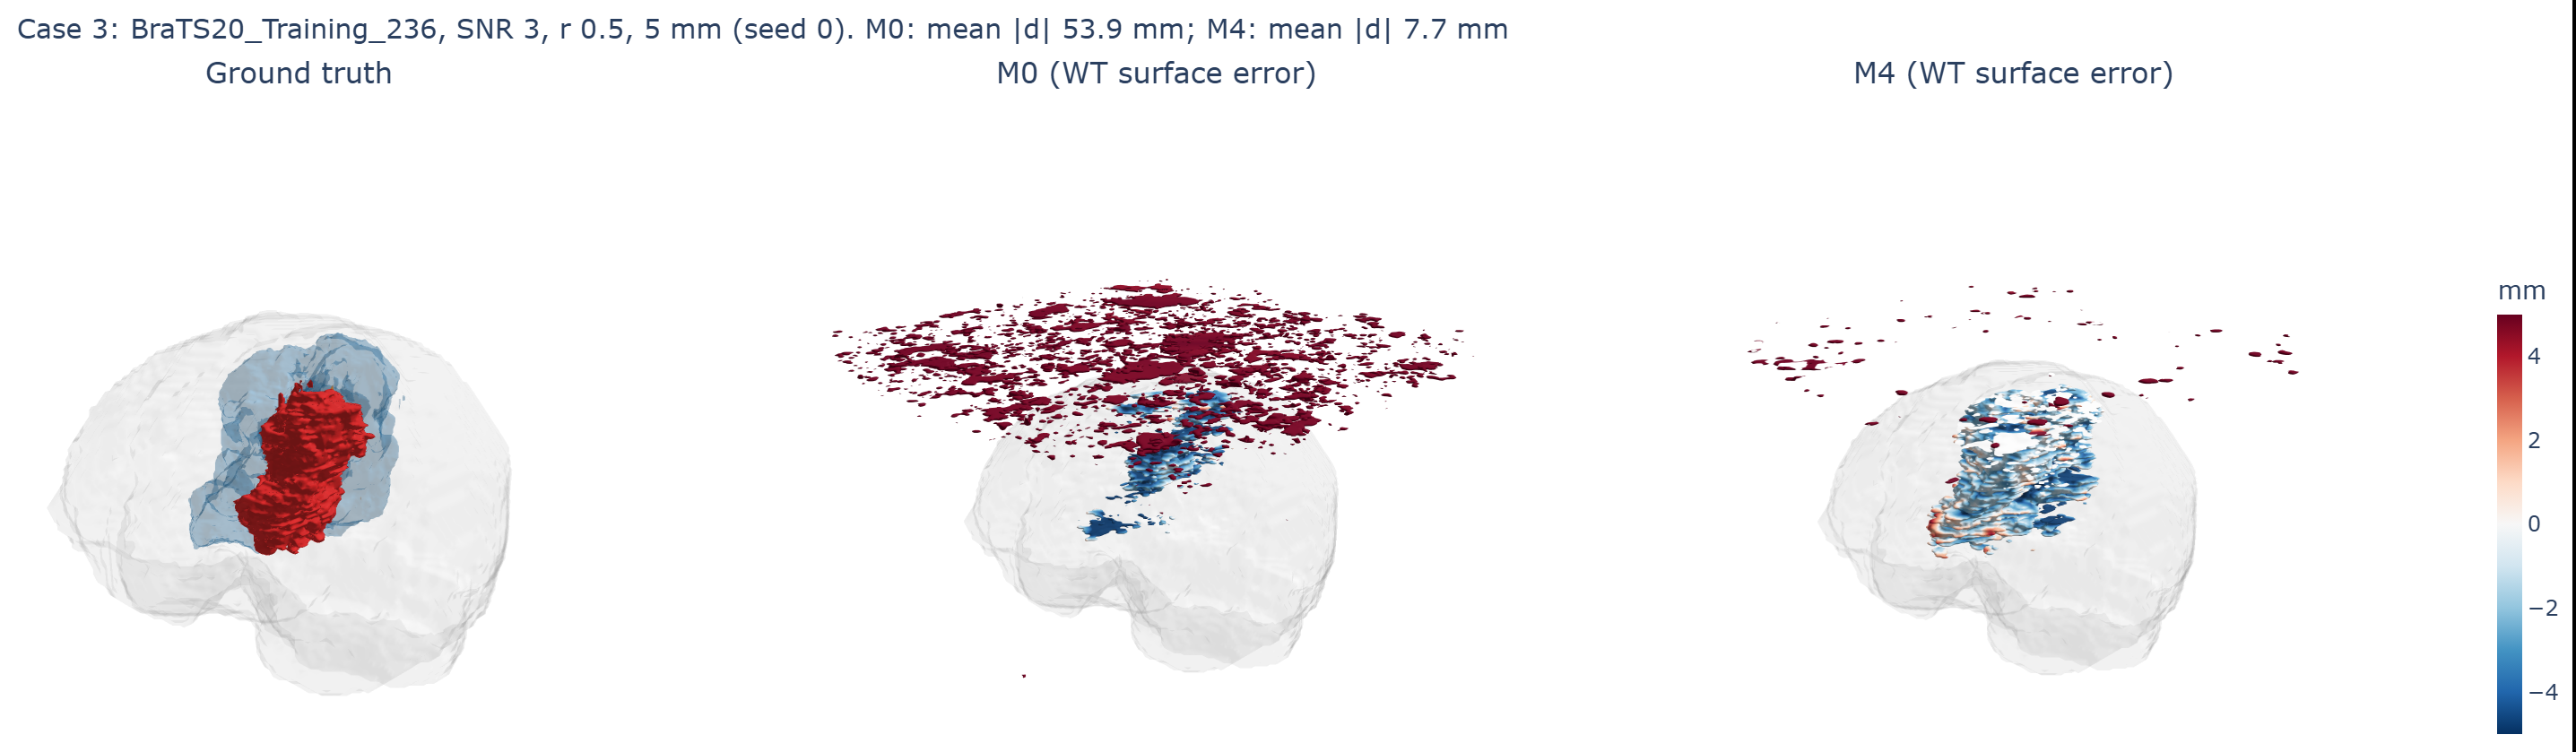
\includegraphics[width=\textwidth]{viz3d_case3_BraTS20_Training_236.png}
\caption{3D comparison at the worst condition, cases 1--3 (HGG small, typical, large), seed 0. Left: ground
truth (WT blue, TC orange, ET red) in a faint brain surface. Middle and right: predicted WT surface of M0 and M4,
coloured by signed distance to the true WT boundary (red outside, blue inside, $\pm5$~mm). Rendered with the
\texttt{viz3d} mesh and surface-error code; interactive versions with all three conditions are produced by
\texttt{python -m viz3d.viewer --compare}.}
\label{fig:viz3dA}
\end{figure*}

\begin{figure*}[t]
\centering
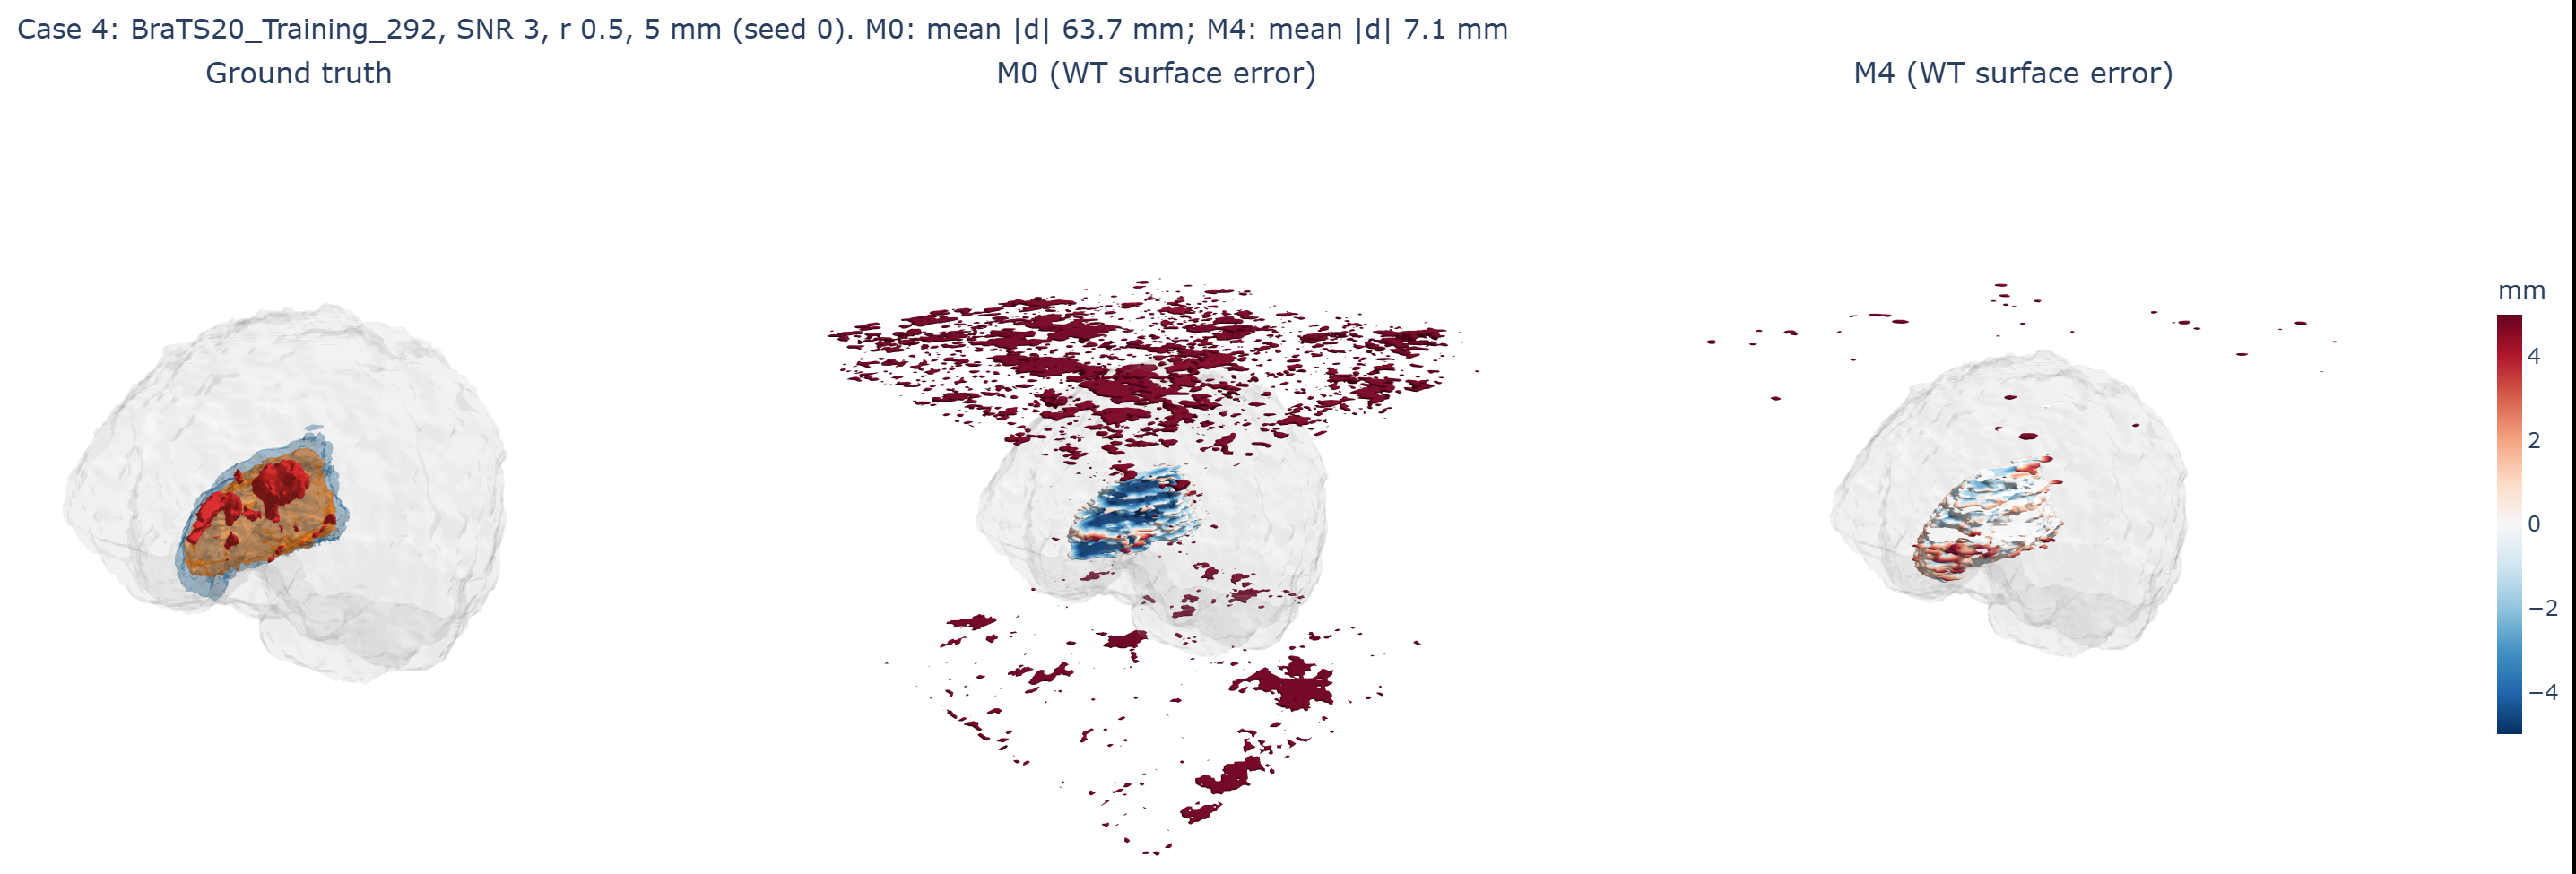
\includegraphics[width=\textwidth]{viz3d_case4_BraTS20_Training_292.png}\\[2pt]
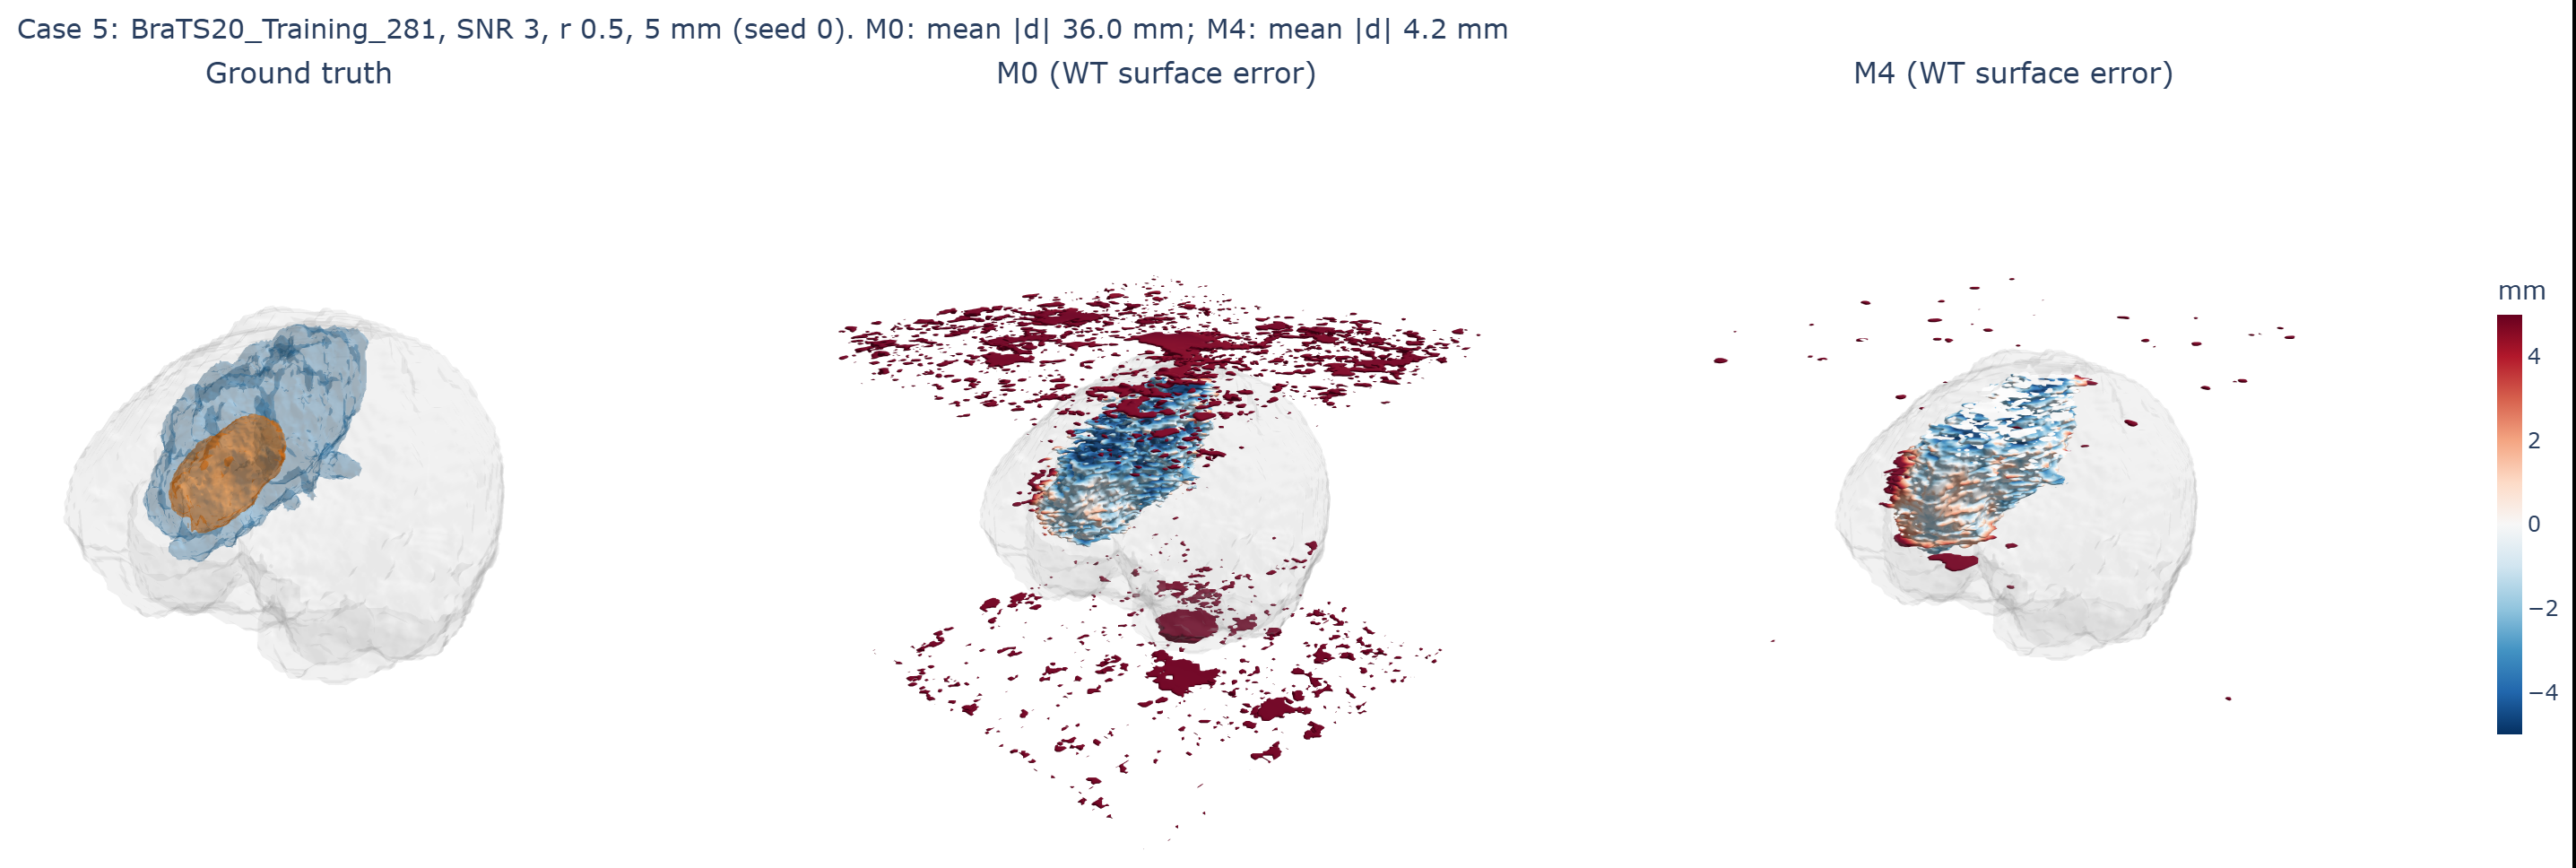
\includegraphics[width=\textwidth]{viz3d_case5_BraTS20_Training_281.png}
\caption{As Fig.~\ref{fig:viz3dA}, cases 4 and 5 (LGG with ET, LGG without ET).}
\label{fig:viz3dB}
\end{figure*}

% ------------------------------------------------------------------------------------------------
\section{Discussion}

\textit{Degradation-aware training is the effect; the architecture is not.} Training on simulated low-field data
raised worst-condition Dice from 0.55 to 0.76--0.77 and removed the clean-trained network's spurious tumor. Given
that training data, splitting the input into bands, as two streams or as extra channels, gave nothing
measurable, and dropping the high band cost nothing. The study was designed to detect an architectural effect:
the hypotheses compared M4 with M1, which shares its training data.

\textit{Why the decomposition did not help.} The split is a fixed, linear, invertible filter, so it offers no
information a plain U-Net lacks; a CNN can learn equivalent filtering in its first layers. Once the network has
seen degraded scans, it learns to discount unreliable fine detail, which is the job the split was meant to do.
That M5 matches M4 is consistent with the high band being mostly degradation from SNR~5 on. The premise of the
design was right; the network did not need the split to act on it.

\textit{Statistical versus practical significance.} H1 and H3 were significant in the wrong direction at about
0.004 Dice. With 74 paired patients a small consistent shift is detectable, but the seed-to-seed spread is
larger, so whether it reflects the architecture or these training runs cannot be told. The pre-registered noise
rule exists for this case.

\textit{Clinical reading.} Part of M0's failure, tumor drawn outside the brain, would be removed by the brain
masking any clinical pipeline applies; the rest would not. Augmented models kept median WT volume error near 7\%
at the worst condition, comparable to their clean-scan error. For scale, expert raters agree on preoperative
glioma volume with ICC(A,1) of 0.92 (grade II--III) to 0.99 (glioblastoma enhancing tumor), and novices on
grade II--III glioma with 0.73~\cite{visser2019interrater}. The augmented models' worst-condition WT ICC
(0.93--0.94) lies at the lower end of the expert range, and M0's (0.74) at novice level, although that study
rated different regions on clinical scans. ET was least robust for every model, as expected for a thin shell: in the synthetic validation a 1~mm boundary
error changed ET volume by a median 48\% but WT by 17\%. A near-zero bias can coexist with large per-patient
error, and a biased method can keep a high ICC (a systematic +17\% error gave ICC 0.957 in the synthetic
validation), so bias, limits of agreement and ICC must be reported together. Every model predicted ET in
patients without ET, so ET presence from these models should not be trusted in LGG.

\textit{Limitations.} The degradation is simulated on magnitude images of high-field data and omits low-field
contrast changes and field inhomogeneity; no labelled low-field tumor scans were available. Augmented models were
tested on the conditions they were trained on, a best case. Networks were 2D, about 4~M parameters, 20 epochs,
one dataset, one cutoff and three seeds. Morphometrics cover seed 0 at three conditions. Pre-registration is an
internal dated log, not a public registry. Predictions were evaluated without post-processing, as pre-specified.

% ------------------------------------------------------------------------------------------------
\section{Conclusion}
Under simulated low-field degradation, training on degraded scans made a U-Net far more robust and removed
spurious tumor, while frequency-band decomposition, as a dual-stream or early-fusion design, added nothing
measurable over a conventional U-Net trained on the same data. With degradation-aware training, tumor volumes
stayed about as reliable at the worst condition as on clean scans; without it, per-patient volumes became
unreliable even though their average error was close to zero. For segmentation on low-field scanners, effort is
better spent on realistic degradation during training than on frequency-specific architectures of this kind.

\bibliographystyle{IEEEtran}
\bibliography{references}

\end{document}
